% ============================================================
%  02_dacta.tex – Chương 2: Đặc tả yêu cầu
% ============================================================
\chapter{Đặc Tả Yêu Cầu}

\section{Mục Đích và Phạm Vi Đặc Tả}

Chương này mô tả các yêu cầu được rút ra từ mã nguồn hiện tại, thay vì mô tả một hệ thống giả định. Mỗi yêu cầu được gắn với tác nhân, đầu vào, kết quả và trạng thái triển khai. Cách tiếp cận này giúp báo cáo có thể dùng làm tài liệu kiểm tra chéo giữa giao diện, API và dữ liệu.

\section{Công Nghệ và Ràng Buộc}

\begin{longtable}{@{}p{0.22\textwidth} p{0.25\textwidth} p{0.45\textwidth}@{}}
  \toprule
  \textbf{Thành phần} & \textbf{Công nghệ} & \textbf{Vai trò trong dự án} \\
  \midrule
  \endhead
  Frontend & React 19, Vite 7, Tailwind CSS 4 & Giao diện mua sắm và khu vực quản trị tùy biến. \\[3pt]
  Backend & Medusa.js 2.15, Node.js 20, TypeScript & API, mô-đun thương mại điện tử, xác thực và nghiệp vụ. \\[3pt]
  Cơ sở dữ liệu & PostgreSQL 15 & Dữ liệu giao dịch, catalog, người dùng và mô-đun tùy biến. \\[3pt]
  Cache và sự kiện & Redis 7 & Cache, event bus, rate limit và đồng bộ giỏ hàng phiên khi được bật. \\[3pt]
  Tìm kiếm & Meilisearch 1.13 & Lập chỉ mục và tìm kiếm sản phẩm theo từ khóa, danh mục, mức giá. \\[3pt]
  Lưu trữ đối tượng & MinIO, giao thức S3 & Ảnh sản phẩm, banner và media quản trị. \\[3pt]
  AI tư vấn & Groq API & Sinh câu trả lời từ FAQ và ngữ cảnh sản phẩm, có fallback khi dịch vụ lỗi. \\[3pt]
  Môi trường & Docker Compose & Khởi tạo PostgreSQL, Redis, Meilisearch và MinIO cục bộ. \\
  \bottomrule
\end{longtable}

Backend yêu cầu Node.js phiên bản từ 20 đến dưới 23; cấu hình của dự án khuyến nghị Node 20 LTS. Frontend gọi API thông qua Medusa JS SDK; địa chỉ backend và publishable key được lấy từ biến môi trường.

\section{Danh Sách Use Case}

\begin{longtable}{@{}p{0.10\textwidth} p{0.25\textwidth} p{0.20\textwidth} p{0.37\textwidth}@{}}
  \toprule
  \textbf{Mã} & \textbf{Use case} & \textbf{Tác nhân} & \textbf{Kết quả mong đợi} \\
  \midrule
  \endhead
  UC01 & Duyệt catalog & Mọi khách & Xem danh sách, danh mục và chi tiết sản phẩm đang bán. \\
  UC02 & Tìm kiếm sản phẩm & Mọi khách & Nhận kết quả theo từ khóa, bộ lọc và thứ tự; fallback khi máy tìm kiếm lỗi. \\
  UC03 & Quản lý giỏ hàng & Mọi khách & Thêm, xóa, đổi số lượng; lưu cục bộ và đồng bộ phiên khi có Redis. \\
  UC04 & Đăng ký/đăng nhập & Khách hàng & Nhận JWT hợp lệ và truy cập chức năng tài khoản. \\
  UC05 & Đặt hàng & Khách hoặc khách hàng & Backend xác minh giá, tồn kho, phí ship, mã giảm giá và tạo đơn. \\
  UC06 & Xem lịch sử đơn & Khách hàng & Chỉ xem các đơn gắn với định danh khách đang đăng nhập. \\
  UC07 & Hộp tự chọn & Mọi khách & Chọn thành phần hộp theo cấu hình sản phẩm và thêm vào giỏ. \\
  UC08 & Tư vấn chatbot & Mọi khách & Trả lời dựa trên FAQ và kết quả catalog; ghi log câu hỏi chưa giải quyết. \\
  UC09 & Quản lý catalog & Nhân viên có quyền & Tạo/sửa sản phẩm, danh mục, công thức và dữ liệu tồn kho. \\
  UC10 & Quản lý đơn hàng & Nhân viên có quyền & Tra cứu chi tiết và cập nhật trạng thái xử lý đơn. \\
  UC11 & Quản lý nội dung & Nhân viên có quyền & Quản lý banner, blog, media, FAQ và các trang chính sách. \\
  UC12 & Báo cáo vận hành & Nhân viên có quyền & Xem chỉ số doanh thu, chi phí, lợi nhuận và dữ liệu tổng hợp. \\
  UC13 & Quản lý người dùng và RBAC & Quản trị viên & Gán vai trò, quyền và giới hạn chức năng theo mô-đun/hành động. \\
  \bottomrule
\end{longtable}

Hình~\ref{fig:use-case-overview} nhóm các use case theo hai tác nhân chính. Đây là sơ đồ tổng quan; các điều kiện và luồng thay thế được đặc tả chi tiết ở các mục tiếp theo.

\begin{diagramcanvas}
\begin{figure}[H]
  \centering
  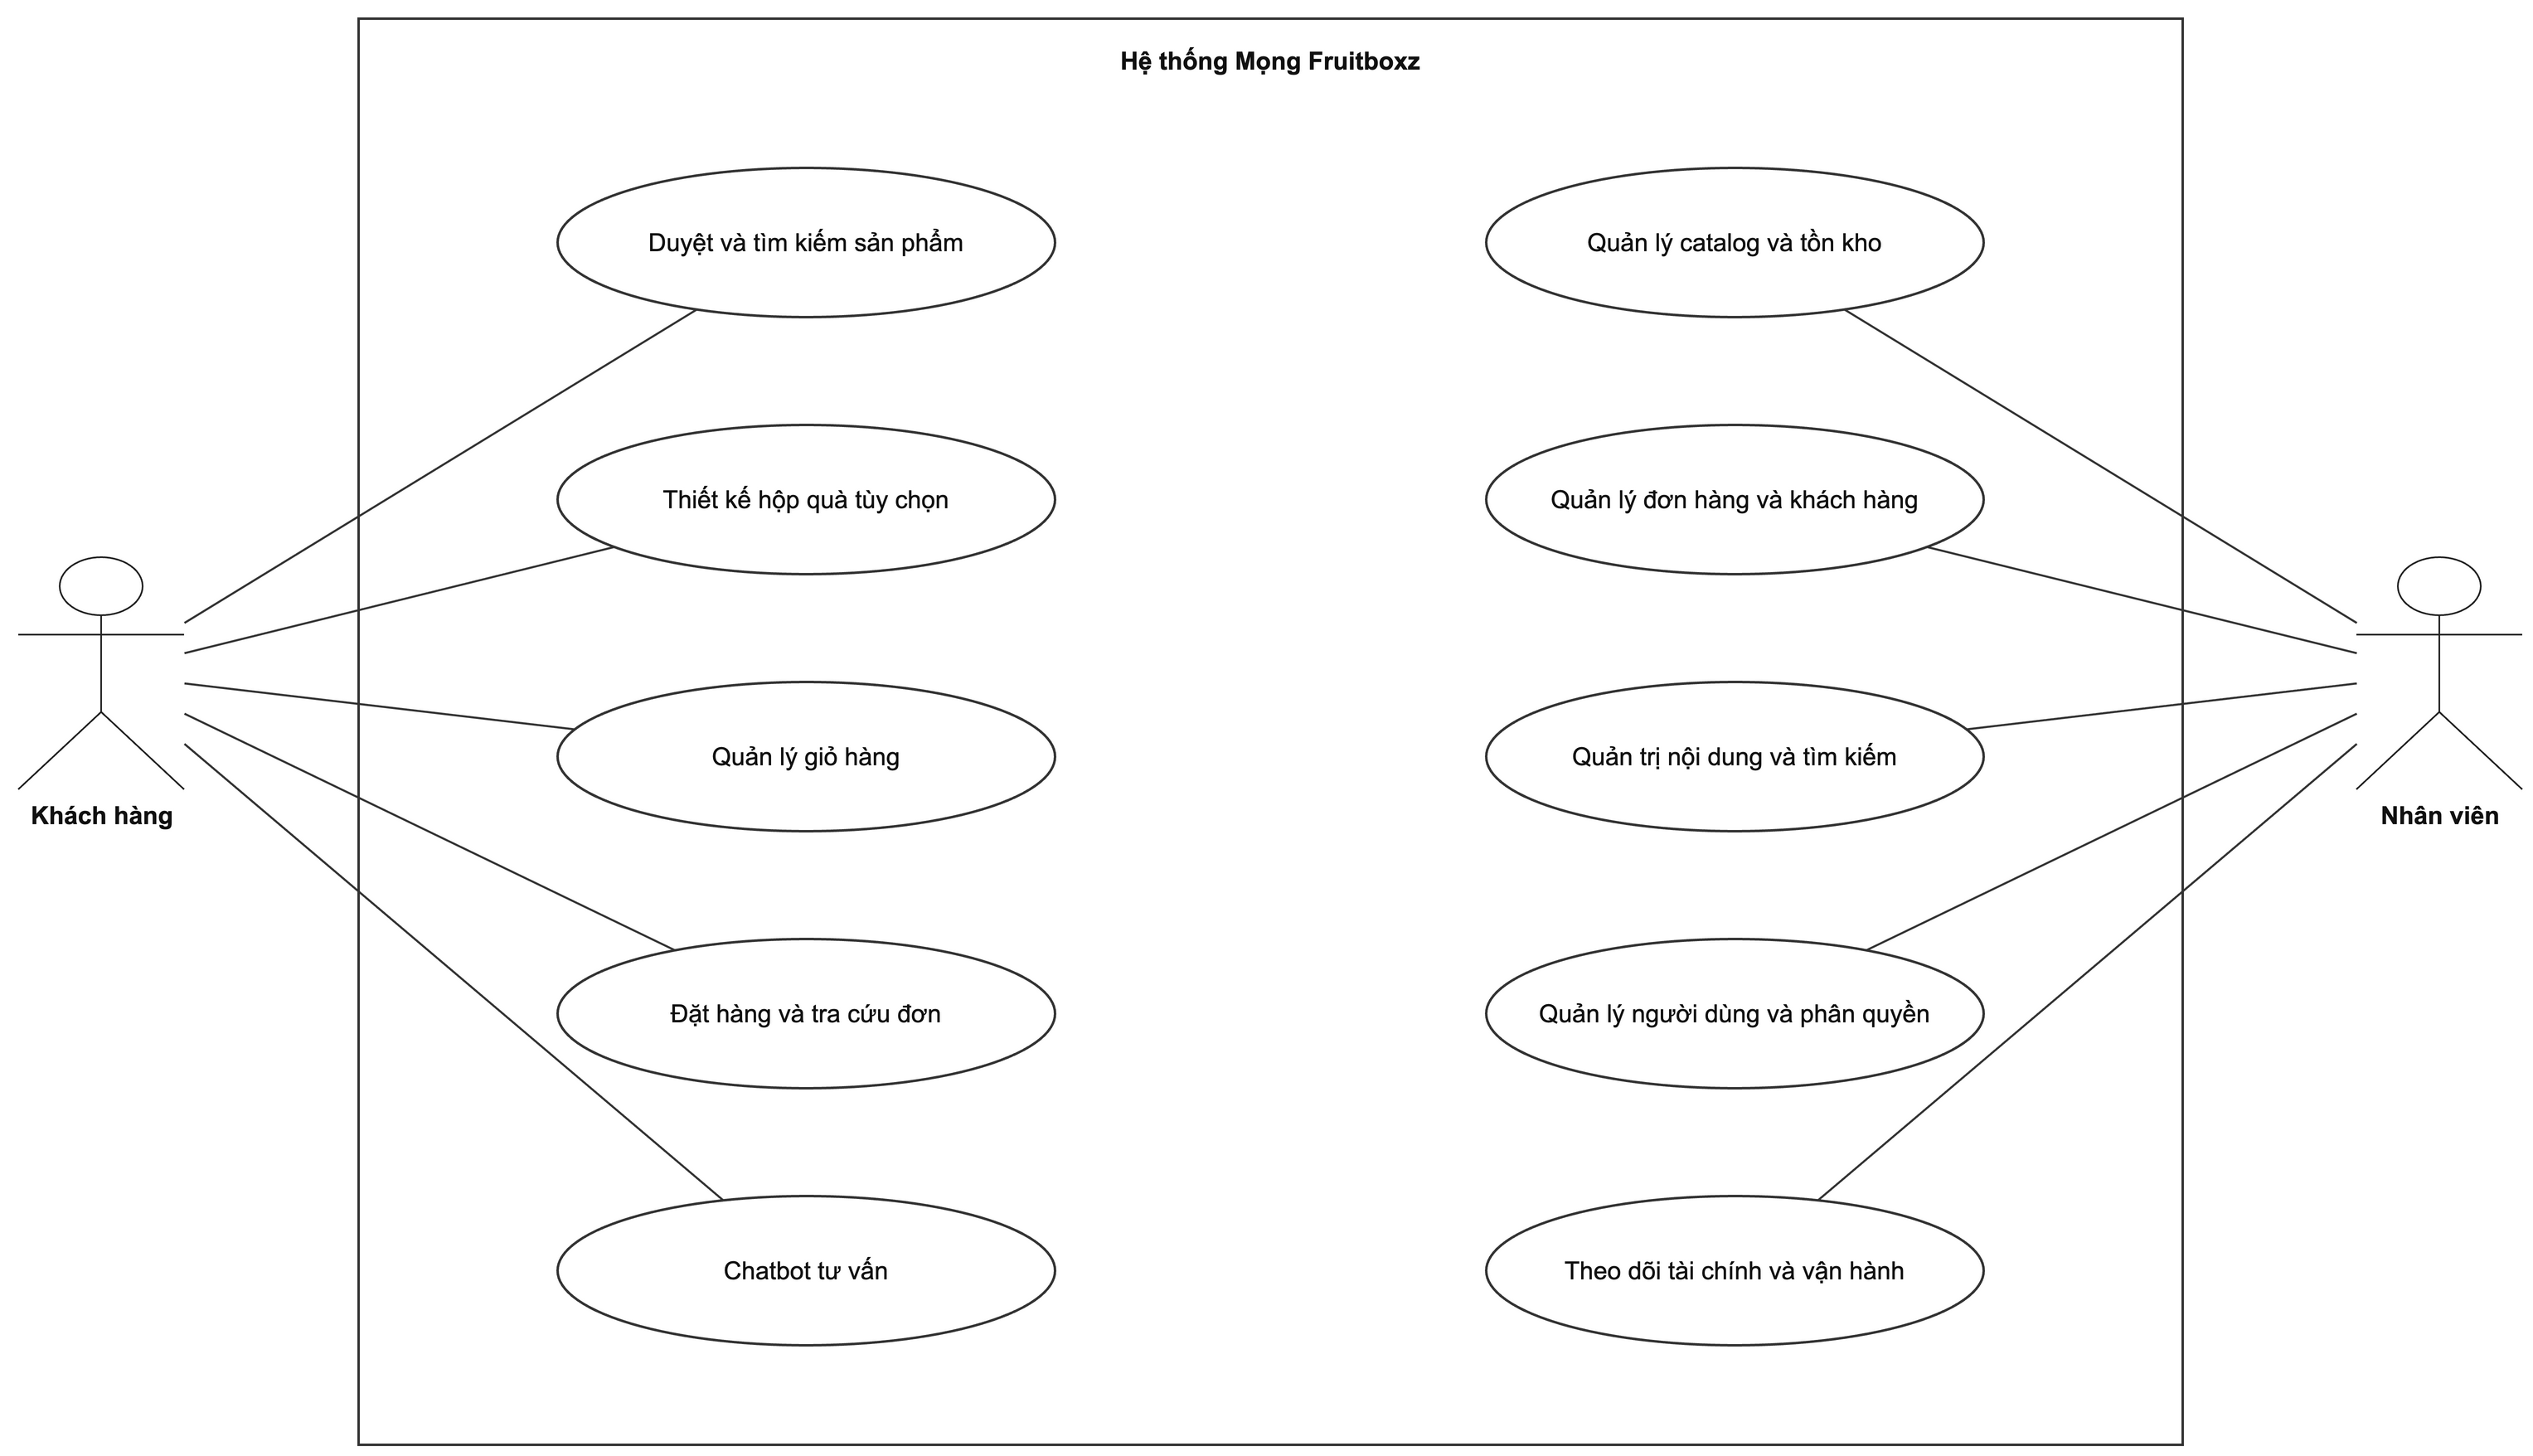
\includegraphics[width=\linewidth,height=0.48\textheight,keepaspectratio]{images/use-case.drawio.png}
  \caption{Use case tổng quan của hệ thống Mọng Fruitboxz}
  \label{fig:use-case-overview}
\end{figure}
\end{diagramcanvas}

\subsection{Quy ước mô hình hóa}

Các sơ đồ trong báo cáo tuân theo quy ước UML được sử dụng trong học phần: tác nhân nằm ngoài biên hệ thống; use case được biểu diễn bằng hình ellipse; quan hệ \textit{include}/\textit{extend} dùng đường nét đứt và mũi tên phụ thuộc; lớp có các ngăn tên--thuộc tính; biểu đồ trình tự đọc từ trên xuống; trạng thái chỉ nối bằng các chuyển tiếp có ý nghĩa nghiệp vụ. Màu sắc chỉ dùng để phân vùng hoặc làm tiêu đề, không mã hóa thêm ngữ nghĩa khi chưa có chú giải. Cách trình bày này giúp người đọc phân biệt rõ sơ đồ phân tích với ảnh giao diện và sơ đồ triển khai.

\section{Đặc Tả Các Luồng Nghiệp Vụ Chính}

\subsection{UC02 -- Tìm kiếm sản phẩm}

\begin{longtable}{@{}p{0.23\textwidth}p{0.69\textwidth}@{}}
  \toprule
  \textbf{Thuộc tính} & \textbf{Đặc tả} \\
  \midrule
  Tác nhân & Mọi khách truy cập. \\
  Tiền điều kiện & Frontend kết nối được backend; Meilisearch là thành phần tối ưu tùy chọn. \\
  Kích hoạt & Người dùng nhập từ khóa hoặc đổi danh mục, mức giá, thứ tự sắp xếp. \\
  Luồng chính & (1) Gửi tiêu chí tìm kiếm; (2) chỉ lấy product \texttt{published}; (3) áp dụng filter, sort và phân trang; (4) trả tên, slug, ảnh, giá, danh mục và trạng thái tồn. \\
  Luồng thay thế & Nếu Meilisearch lỗi hoặc chưa cấu hình, backend dùng Medusa Query, chuẩn hóa chuỗi và lọc catalog tại ứng dụng. \\
  Hậu điều kiện & Danh sách kết quả và tổng số bản ghi khớp tiêu chí được hiển thị; dữ liệu không bị thay đổi. \\
  \bottomrule
\end{longtable}

\subsection{UC03 -- Quản lý giỏ hàng}

\begin{longtable}{@{}p{0.23\textwidth}p{0.69\textwidth}@{}}
  \toprule
  \textbf{Thuộc tính} & \textbf{Đặc tả} \\
  \midrule
  Tác nhân & Mọi khách truy cập. \\
  Tiền điều kiện & Sản phẩm có biến thể hợp lệ và còn khả năng mua. \\
  Luồng chính & Thêm sản phẩm, đổi số lượng, chọn dòng hàng hoặc xóa; reducer cập nhật trạng thái và lưu \techterm{localStorage}. \\
  Đồng bộ & Mỗi trình duyệt có session ID; frontend thử đồng bộ qua \texttt{/store/session-cart/:id} khi Redis hoạt động. \\
  Luồng suy giảm & Redis lỗi không chặn mua hàng; localStorage trở thành nguồn dữ liệu hoạt động. Ảnh cũ được đối chiếu lại thumbnail từ catalog. \\
  Hậu điều kiện & Tổng số lượng và tạm tính được cập nhật; giỏ còn tồn tại sau khi tải lại trang. \\
  \bottomrule
\end{longtable}

\subsection{UC05 -- Đặt hàng}

\begin{longtable}{@{}p{0.23\textwidth}p{0.69\textwidth}@{}}
  \toprule
  \textbf{Thuộc tính} & \textbf{Đặc tả} \\
  \midrule
  Tác nhân & Khách vãng lai hoặc khách hàng đã đăng nhập. \\
  Tiền điều kiện & Giỏ có ít nhất một dòng hàng; tên, điện thoại và địa chỉ hợp lệ. Email là tùy chọn. \\
  Đầu vào & \texttt{variant\_id}, số lượng, thông tin người nhận, địa chỉ hoặc tọa độ, mã khuyến mãi; backend hỗ trợ khóa idempotency tùy chọn. \\
  Luồng chuẩn bị & Người dùng có thể cho phép định vị. Frontend gọi reverse geocode để điền địa chỉ; mỗi khi địa chỉ/tọa độ thay đổi, hiệu ứng debounce 300 ms tự gọi \texttt{/store/shipping/quote} và cập nhật phí, chế độ tính cùng khoảng cách ước lượng. \\
  Luồng chính & (1) Xác thực payload; (2) nếu có khóa idempotency thì tìm đơn đã xử lý; (3) tải lại biến thể và giá VND; (4) tính nhu cầu BOM, kiểm tra tồn; (5) tính lại ship và promotion tại server; (6) tạo order \texttt{pending} và mã \texttt{MONG-...}; (7) phát \texttt{order.placed}; (8) trả order và bảng tổng hợp. \\
  Luồng lỗi & Từ chối khi biến thể không tồn tại, thiếu giá, thiếu nguyên liệu, promotion không hợp lệ hoặc dữ liệu giao hàng sai. Nếu reverse geocode lỗi, giữ tọa độ và yêu cầu người dùng bổ sung địa chỉ; nếu API quote lỗi, frontend dùng ước lượng cục bộ. \\
  Quy tắc tin cậy & Không dùng giá/tổng tiền gửi từ trình duyệt làm nguồn chuẩn. Phí giao hàng và giảm giá được tính lại ở backend; idempotency chỉ có hiệu lực khi client cung cấp khóa. \\
  Hậu điều kiện & Order và metadata giao hàng được lưu; frontend xóa giỏ và hiển thị mã đơn, tổng thanh toán cùng QR chuyển khoản. \\
  \bottomrule
\end{longtable}

Hình~\ref{fig:checkout-activity} mô tả luồng nghiệp vụ từ góc nhìn trách nhiệm; Hình~\ref{fig:shipping-quote-sequence} mô tả bước định vị và báo phí; Hình~\ref{fig:checkout-flow} mô tả các bước kiểm tra khi tạo đơn. Như vậy UC05 được đặc tả bằng cả bảng văn bản, biểu đồ hoạt động và các sơ đồ luồng, phù hợp cách mô hình hóa chức năng--hành vi trong slide học phần.

\subsubsection{Bảng quyết định phí giao hàng}

\begin{longtable}{@{}p{0.29\textwidth}p{0.25\textwidth}p{0.38\textwidth}@{}}
  \toprule
  \textbf{Điều kiện} & \textbf{Chế độ} & \textbf{Kết quả} \\
  \midrule
  Chưa có địa chỉ/tọa độ & \texttt{fallback-empty} & Dùng phí Hà Nội mặc định để tạm tính. \\
  Ngoài Hà Nội & \texttt{static-non-hanoi} & Dùng mức phí ngoài Hà Nội từ cấu hình. \\
  Quận thuộc danh sách miễn phí & \texttt{district-free} & Phí giao hàng bằng 0. \\
  Khớp quận hoặc có tọa độ & \texttt{distance-estimate} & Khoảng cách đường đi ước lượng bằng Haversine $\times 1{,}3$; phí = phí nền + đơn giá/km, làm tròn nghìn và chặn min--max. \\
  Có địa chỉ Hà Nội nhưng không khớp quận & \texttt{static-hanoi} & Dùng phí Hà Nội mặc định. \\
  API quote không khả dụng & \texttt{fallback} ở frontend & Ước lượng cục bộ theo quận đã nhận diện; nếu không nhận diện được thì dùng phí mặc định. \\
  \bottomrule
\end{longtable}

\subsection{UC08 -- Chatbot tư vấn}

\begin{longtable}{@{}p{0.23\textwidth}p{0.69\textwidth}@{}}
  \toprule
  \textbf{Thuộc tính} & \textbf{Đặc tả} \\
  \midrule
  Tác nhân & Mọi khách truy cập. \\
  Đầu vào & Câu hỏi tự nhiên; không nhận dữ liệu đơn hàng hoặc thông tin thanh toán. \\
  Luồng chính & Chuẩn hóa câu hỏi, tìm FAQ và tối đa bốn sản phẩm liên quan, tạo prompt có ngữ cảnh rồi gọi Groq. \\
  Ràng buộc & Không bịa sản phẩm, không tiết lộ prompt, không truy cập dữ liệu cá nhân; có rate limit theo IP và cache câu trả lời. \\
  Luồng thay thế & Trả FAQ trực tiếp; nếu AI lỗi thì dùng kết quả catalog hoặc hướng dẫn liên hệ hotline. \\
  Hậu điều kiện & Nội dung trả lời, chế độ phản hồi và trạng thái resolved được ghi vào chatbot log. \\
  \bottomrule
\end{longtable}

\subsection{UC13 -- Phân quyền quản trị}

\begin{longtable}{@{}p{0.23\textwidth}p{0.69\textwidth}@{}}
  \toprule
  \textbf{Thuộc tính} & \textbf{Đặc tả} \\
  \midrule
  Tác nhân & Người dùng quản trị đã được cấp tài khoản. \\
  Tiền điều kiện & JWT admin hợp lệ; metadata chứa danh sách role hiện hành. \\
  Luồng chính & Tải permission; giao diện dùng \texttt{RequirePermission}; backend ánh xạ route và HTTP method sang \texttt{module.action}, sau đó cho phép hoặc trả 403. \\
  Quy tắc & Kiểm tra quyền bắt buộc ở backend; ẩn menu chỉ là biện pháp UX. Super admin dùng permission đại diện \texttt{*}. \\
  Hậu điều kiện & Chỉ các route và thao tác được cấp quyền mới thực thi; thay đổi role phản ánh khi tải lại quyền. \\
  \bottomrule
\end{longtable}

\section{Truy Vết Yêu Cầu Sang Thiết Kế}

\begin{longtable}{@{}p{0.15\textwidth}p{0.27\textwidth}p{0.25\textwidth}p{0.25\textwidth}@{}}
  \toprule
  \textbf{Use case} & \textbf{Mô hình hành vi} & \textbf{Thành phần thực thi} & \textbf{Bằng chứng giao diện} \\
  \midrule
  UC02 & Use case tổng quan & Search API, Meilisearch, fallback Query & Hình~\ref{fig:ui-discovery} \\
  UC03 & Activity checkout, bước chuẩn bị giỏ & \texttt{CartContext}, session cart & Hình~\ref{fig:ui-assist-checkout} \\
  UC05 & Activity, luồng định vị/báo phí, luồng tạo đơn, state order & Checkout UI/API, geocode, quote, Ingredient, Order, Event Bus & Hình~\ref{fig:ui-assist-checkout} \\
  UC08 & Sequence chatbot & Chatbot API, FAQ/catalog retrieval, Groq & Hình~\ref{fig:ui-assist-checkout} \\
  UC09--UC13 & Module, class, ERD và deployment & Admin routes, RBAC, module service & Hình~\ref{fig:ui-admin-overview} và \ref{fig:ui-admin-operations} \\
  \bottomrule
\end{longtable}

\section{Yêu Cầu Phi Chức Năng}

\begin{longtable}{@{}p{0.22\textwidth} p{0.70\textwidth}@{}}
  \toprule
  \textbf{Thuộc tính} & \textbf{Yêu cầu và cách kiểm chứng} \\
  \midrule
  \endhead
  Hiệu năng & Route giao diện được tách bundle; ảnh tải lười; tìm kiếm ưu tiên chỉ mục Meilisearch và có phân trang. \\
  Tin cậy & Checkout dùng khóa idempotency; giá được xác minh tại server; cache, Redis và tìm kiếm đều có phương án suy giảm chức năng. \\
  Bảo mật & JWT tách customer/admin; backend kiểm tra RBAC; payload được xác thực; secret lấy từ biến môi trường. \\
  Khả dụng & Luồng browse--cart--checkout có thông báo loading/error; các trang chính hoạt động ở kích thước desktop và mobile. \\
  Bảo trì & API chia namespace, nghiệp vụ chia module, migration đi cùng module và thành phần giao diện được tái sử dụng. \\
  Quan sát & Lỗi API có mã trạng thái rõ; chatbot lưu log câu hỏi; production cần bổ sung structured log và metric. \\
  \bottomrule
\end{longtable}

\section{Yêu Cầu Dữ Liệu và Kiểm Tra Hợp Lệ}

\begin{itemize}[leftmargin=2em, itemsep=4pt]
  \item Định danh sản phẩm và biến thể phải tồn tại tại thời điểm checkout.
  \item Số lượng mua phải là số nguyên dương và không vượt quá lượng nguyên liệu khả dụng.
  \item Giá đơn hàng luôn được lấy từ backend và dùng tiền tệ VND.
  \item Email, số điện thoại, địa chỉ và payload contact/chatbot được kiểm tra qua middleware Zod.
  \item Khách vãng lai không được tự động gắn đơn vào tài khoản đã tồn tại chỉ dựa trên email.
  \item API admin yêu cầu xác thực; các mô-đun nhạy cảm yêu cầu thêm quyền RBAC tương ứng.
\end{itemize}

\section{Tiêu Chí Chấp Nhận}

\begin{longtable}{@{}p{0.28\textwidth} p{0.64\textwidth}@{}}
  \toprule
  \textbf{Nhóm} & \textbf{Tiêu chí} \\
  \midrule
  \endhead
  Catalog & Sản phẩm xuất bản hiển thị đúng tên, ảnh, giá, biến thể và danh mục. \\
  Checkout & Không tạo đơn nếu giá/tồn kho không hợp lệ; tổng tiền thể hiện được giảm giá và phí giao hàng. \\
  Bảo mật & Route admin từ chối người chưa xác thực; người thiếu quyền nhận mã 403. \\
  Khả dụng & Giỏ hàng vẫn hoạt động khi Redis lỗi; tìm kiếm có kết quả fallback khi Meilisearch lỗi. \\
  Quản trị & Thay đổi catalog/nội dung được phản ánh ở frontend và chỉ mục liên quan được vô hiệu hóa hoặc cập nhật. \\
  Responsive & Các luồng mua hàng chính sử dụng được trên màn hình desktop và thiết bị di động. \\
  \bottomrule
\end{longtable}

\section{Giới Hạn Phạm Vi Hiện Tại}

Phiên bản được rà soát chưa tích hợp cổng thanh toán trực tuyến; đơn mới được ghi nhận với trạng thái \texttt{not\_paid}. Subscriber email mới ghi nội dung ra log thay vì gửi qua nhà cung cấp thực. Dự án chưa có bộ kiểm thử tự động và pipeline CI rõ ràng. Những nội dung này được xem là hướng hoàn thiện, không được tính là chức năng đã triển khai đầy đủ.
